\section{Extended systems modeling technique}
\label{section:foundation}

Our approach to rapid multi-objective transportation and power system scenario modeling and evaluation is based on emergent property estimation techniques \cite{hackenberg2012towards} that have been integrated into a rapid prototyping method for the smart energy systems domain~\cite{hackenberg2014rapid}. An instantiation of the underlying systems modeling technique for the intelligent transportation systems (ITS) domain was proposed in~\cite{ascher2014early}, which enables the formulation of multi-objective traffic flows as an optimal control problem over state variables (e.g.\ vehicle position), control variables (e.g.\ vehicle speed and route), constraints (e.g.\ collision avoidance) and objectives (e.g.\ energy efficiency). Finally, the approach employs a generic solver that utilizes stochastic (i.e.\ Monte-Carlo) optimization techniques.

Originally, the modeling technique allowed one to express static interaction between components (e.g.\ vehicles and controllers) based on input/output (I/O) ports (e.g.\ vehicle speed) and channels (e.g.\ vehicle speed from controller to vehicle and vice versa). In this work we extend the underlying systems modeling technique to cope with changing scenario configurations as well as the dynamic interaction between transportation and power system (i.e.\ vehicle and charging station) as shown in Figure~\ref{fig:meta_model}.

\begin{figure}[h]
	\centering
	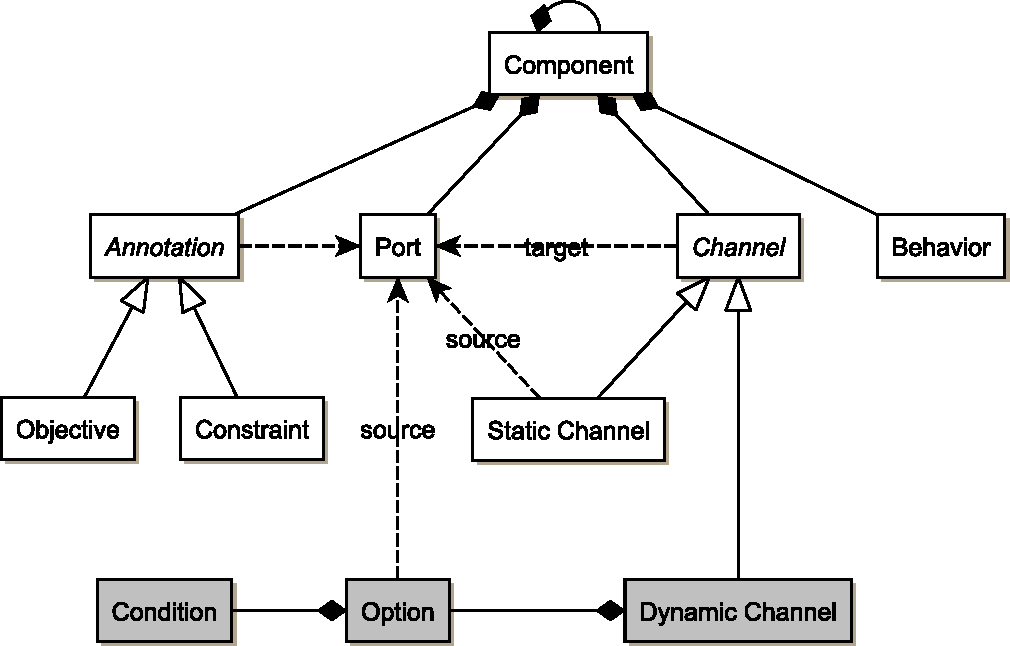
\includegraphics[width=\columnwidth]{../gfx/meta_model.pdf}
	\caption{Meta-model of the underlying systems modeling technique}%extended with parameters and dynamic channels.
	\label{fig:meta_model}
\end{figure}

The core element of the underlying systems modeling technique is the \textit{component} (e.g.\ vehicle and charging station). Components can be either atomic (i.e.\ no subcomponent) or composite (i.e.\ one or more subcomponents) depending on their complexity. Components can be configured in their specific occurrence (e.g.\ vehicle length and weight). Possible interactions between components can be specified in terms of \textit{ports} and \textit{channels}. Ports can be either input (e.g.\ vehicle speed) or output (e.g.\ vehicle position) with respect to some component (e.g.\ vehicle). In contrast, channels specify the flow of information between ports. We distinguish between \textit{static} and \textit{dynamic channels}. Static channels define information flow from a fixed source to a fixed target port. Instead, dynamic channels define information flow from a number of possible source ports to a fixed target port. The source ports are modeled in terms of an ordered list of \textit{options} and \textit{conditions}. During simulation the first option is selected whose condition is satisfied. Finally, component \textit{behaviors} and \textit{annotations} can be specified. Behaviors calculate the component state and information flow during simulation. Annotations defined the \textit{constraints} and \textit{objectives} of the optimization problem instead. Thereby, annotations refer to respective boolean (for constraints) and numeric (for objectives) output ports.